\documentclass[12pt]{article}
\usepackage{url, hyperref, geometry, amsmath, amsfonts, amsthm, nicefrac, graphicx}
\usepackage[table,xcdraw]{xcolor}
\usepackage{graphicx}

\geometry{paper=letterpaper, textheight=9.0in, textwidth=6.5in}

\hypersetup{ 
pdftitle = {Artificial Intelligence 600.335, Spring 2015, Homework 2},
pdfauthor = {Corbin Rosset}
}

\newcommand{\ttt}[1]{\texttt{#1}}
\newcommand{\n}{\vspace{5mm}}

\makeatletter
\newcommand{\exercise}[1]{\par\vspace{4ex}\normalfont\normalsize\noindent
\textbf{\large Problem #1}\par\nobreak\@afterindentfalse\@afterheading\vspace{.75ex}}
\makeatother

\newenvironment{questionList}{
\newcounter{ctr}
\begin{list}{\textbf{Question \arabic{ctr}.} \\ \\ }
  {\usecounter{ctr}}
  }{
\end{list}
}



\title{Homework 2: Adversarial Search\\ \normalsize\emph{Artificial Intelligence 600.335, Spring 2015}}
\date{\emph{due date:} February 27th, 2015}
\author{Corbin Rosset}

\begin{document}
\maketitle



\section{Written Questions}

\exercise{1}
Below are the results of the number of nodes expanded in total for each board size and AI construct at each depth. This was averaged over two games each, one with MiniMax (MM) as black, and then again with MM as white. 

\begin{table}[h]
\begin{tabular}{|l|l|l|l|l|l|l|}
\hline
Depth & 4x4 MM & 4x4 AB & 6x6 MM    & 6x6 AB    & 8x8 MM     & 8x8 alphaBeta \\ \hline
1     & 112    & 112    & 889       & 889       & 5755       & 5755          \\ \hline
2     & 235    & 235    & 7850      & 7850      & 51825      & 51825         \\ \hline
3     & 724    & 665    & 40439     & 36945     & 792,929    & 719,976       \\ \hline
4     & 2439   & 1939   & 293,401   & 218,819   & 10,033,731 & 7,975,341     \\ \hline
5     & 2710   & 1543   & 1,183,820 & 658,641   & 51,945,299 & 31,047,857    \\ \hline
6     & 8509   & 4000   & 6,361,825 & 2,857,710 & *          & *             \\ \hline
\end{tabular}
\end{table}

* meaning the game did not terminate in a reasonable amount of time (30 minutes). I predict the nodes expanded would be in the hundreds of millions, if not around 1 billion.  
\exercise{2}
Below is the table for running MiniMax vs. AlphaBeta both at maxDepth of 7 on a 4x4 board. The entries were averaged with the AlphaBeta vs. MiniMax game. It took only 10 turns total (5 by each player) for white to win. 
\begin{table}[h]
\begin{tabular}{|l|l|l|l|l|}
\hline
Turn & MM nodes & AB nodes & MM time (ms) & AB time (ms) \\ \hline
0    & 6255     & 2101     & 59           & 35           \\ \hline
1    & 970      & 361      & 2            & 1            \\ \hline
2    & 324      & 135      & 0            & 0            \\ \hline
3    & 54       & 35       & 0            & 0            \\ \hline
4    & 1        & 1        & 0            &  0            \\ \hline
\end{tabular}
\end{table}

Below is a similar table, but for a maxDepth of 5 on a 6x6 board, averaged with AlphaBeta being black and then white. 

\begin{table}[h]
\begin{tabular}{|l|l|l|l|l|}
\hline
Turn & MM nodes & AB nodes & MM time (ms) & AB time (ms) \\ \hline
0    & 344,147   & 195,856   & 1,697         & 663          \\ \hline
1    & 167,885  & 91,261    & 700          & 256          \\ \hline
2    & 241,605   & 126,506   & 953          & 337          \\ \hline
3    & 158,064   & 85,950    & 591          & 219          \\ \hline
4    & 104,645  & 56,340   & 350          & 134          \\ \hline
5    & 86,905   & 52,751   & 564          & 125          \\ \hline
6    & 51,949   & 32,276   & 282          & 71           \\ \hline
7    & 17,979   & 10,642   & 150          & 19           \\ \hline
8    & 8,031     & 5,406     & 42           & 12           \\ \hline
9    & 2,041    & 1,248     & 17           & 1            \\ \hline
10   & 567      & 402      & 5            & 0            \\ \hline
\end{tabular}
\end{table}

And lastly, here is the graph for an 8x8 board with depth 3. (For some reason it appears on the next page?). 

\begin{table}[h]
\begin{tabular}{|l|l|l|l|l|}
\hline
Turn & MM nodes & AB nodes & MM time (ms) & AB time (ms) \\ \hline
0    & 53459.5  & 47448    & 837.5        & 539.5        \\ \hline
1    & 31847    & 27259.5  & 438          & 256.5        \\ \hline
2    & 44993    & 40319.5  & 582.5        & 371          \\ \hline
3    & 51307.5  & 45182.5  & 699          & 410.5        \\ \hline
4    & 60637    & 53093.5  & 808.5        & 477.5        \\ \hline
5    & 75921    & 66038.5  & 968          & 580          \\ \hline
6    & 62228    & 53765    & 767          & 454          \\ \hline
7    & 72574    & 62409    & 850.5        & 502.5        \\ \hline
8    & 56641.5  & 49913.5  & 624.5        & 374.5        \\ \hline
9    & 65551.5  & 62643.5  & 773          & 593.5        \\ \hline
10   & 53620    & 52284    & 632          & 521.5        \\ \hline
11   & 43863.5  & 42663    & 476.5        & 395          \\ \hline
12   & 34856    & 33997    & 353.5        & 311.5        \\ \hline
13   & 25530    & 25027    & 243.5        & 216          \\ \hline
14   & 22195.5  & 21632    & 185          & 165.5        \\ \hline
15   & 14083.5  & 13750.5  & 102.5        & 91.5         \\ \hline
16   & 9206     & 8919     & 58.5         & 52           \\ \hline
17   & 7179.5   & 6918     & 40.5         & 35           \\ \hline
18   & 4484.5   & 4284     & 21           & 19           \\ \hline
19   & 1569.5   & 1396     & 5            & 3.5          \\ \hline
20   & 843      & 732.5    & 2.5          & 1.5          \\ \hline
21   & 255.5    & 231.5    & 0            & 0            \\ \hline
22   & 71.5     & 58       & 0            & 0            \\ \hline
23   & 6.5      & 6.5      & 0            & 0            \\ \hline
24   & 4.5      & 4.5      & 0            & 0            \\ \hline
\end{tabular}
\end{table}

\exercise{3}

There are a couple of points to make about these algorithms. Firstly, they do not scale very well with larger boards because the branching factors cause the exponential growth to be unbearable past a depth of say 7. To compensate, we must shorten the depth for the larger boards, which really means the AI constructs are becoming literally more shortsighted with larger branching factors. This shows that pruning becomes all the more important with higher branching factors because we need to eliminate as many "junk" nodes as possible so we can have time to explore more promising nodes, or we won't make any progress. However, if our heuristic is imperfect, we may be eliminating really good moves by incorrectly pruning them. Also, There are clever tricks to node ordering that can be done to bring alpha-beta pruning closer to the theoretical limit of square rooting the branching factor, but at least in my algorithm, alpha-beta seems to be getting pretty close to that limit anyway, barring consideration of the first few moves, which are special cases. It is true that if alpha-beta was given the same amount of time as minimax, alpha beta would be able to go about twice as deep. One move ordering strategy could have been try first to take pieces with double jumps (a pseudo-"kill" strategy), then moves that take just one piece. This is supported by the first table, which shows alpha beta expanding about $0.6$ or $0.7$ as many nodes as minimax. This ratio approaches one half as the depth increases, which is to be expected since pruning is more likely at greater depths because pruning operates on the depth-first path taken so far. 

Looking now at the tables, we immediately see a commonality between all of them: generally more nodes are expanded in the earlier moves. This isn't entirely monotonic, due to the restrictive nature of the game's opening moves. Depending on which piece Black removes from the board first, there are relatively few moves white can take in response, since it must be $adjacent$ to Black's removed piece. If black takes a corner piece, there are only two moves white can make, which heavily restricts the number of nodes expanded on the 1st turn (turn 0 being the opening turn). That is why there is usually an initial drop (by a factor of 2) of the number nodes expanded in turn 1. Then in turn 2, the expansions ramp up again as the game has about twice as many response moves again. Thus it is really those corner removals by Black on turn 0 that restrict expansion. 

In the middle of the game, especially for the 8x8 board, we a see an almost sinusoidal oscillation in node expansion by both alpha beta and minimax, which reverts to a monotonically decreasing polynomial (or exponential, difficult to tell when you plot it) by around move 9. When you actually look at the boards generated at these turns, you notice voids or gaps opening up in which one player clearly has more moves than the other. For example examine: 


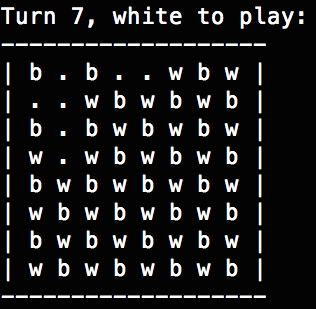
\includegraphics{./images/example.png}

Notice that black has many more moves than white based on the structure of the holes that have emerged (white only has 2 moves). This with such a disparity in the initial number of possible moves between players it is not suprising that the number of nodes expanded fluctuates. Remember, for each available move, there is a whole tree below it that can be expanded. As the board becomes more developed and the holes start becoming less contiguous, then the branching factors become more equitable between players and node expansion stabilizes to its predicted monotonic function. 


Notice that the relationship between runtime and node expansion is about linear, which is to be expected since expansion is a metric for "work" since we can expect each node to have roughly the same branching factor. 

Also note one pattern which seems to have emerged: with my heuristic, as you increase the board size from 4 to 6 to 8, the number of turns played until the game is won increases by about a factor of 2 (5 turns, 11 turns, 25 turns). This could be exponential (there really isn't enough data), but it's an interesting point to investigate. This could have something to do with the next phenomenon, which is the game seems to degenerate into "rank" of alternating columns of pieces and empty tiles: 

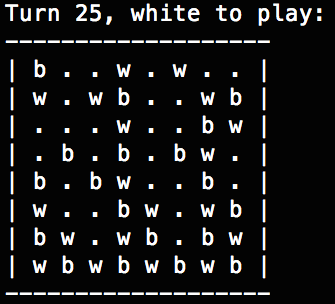
\includegraphics{./images/example1.png}

In the figure above you can see that pieces tend to cluster around the edges, and in columns of thickness 2 separated by "trenches" of empty tiles of thickness 2. Thus there is a pattern of pieces  back to back that can attack each other by landing in one of the trenches. This makes sense given my heuristic because each AI is trying to either put itself against a wall or surround itself with enemies. It turns out when both players try to do this, they cluster together into ranks that  fall apart like dominos once one person makes the first move to break up the rank. Notice that if I had implemented a utility that was weighted also by taking double jumps (to take two opponent pieces in one move) I predict this phenomenon would be avoided. Indeed, in the board above there exists even a triple jump. 

The following example is even more illustrative: 

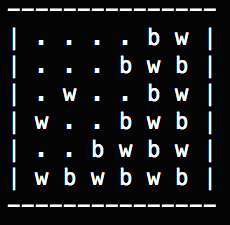
\includegraphics{./images/example2.png}

This is an example where white won being an alpha beta player with depth 6 versus an black minimax player of depth 4. White has positioned itself so that it is always in a position to take black, but black cannot take white. 

Towards the end of the game moves are made very quickly because either there are few pieces are pieces are isolated to the point where they cannot possibly interact anymore. Overall, the algorithms do horribly with just small increments in depth or board size, but this shortcoming can be harmless if a good evaluation heuristic is used. Like I mentioned before, my very simple heuristic is able to beat a random player 75 percent of the time. While not great, it isn't difficult to believe that more advantageous heuristics are achievable, while greater depths simply aren't achievable. Thus heuristics are of greater value to an AI than the number of states it can explore, which makes sense because AI is all about the quality of decisions you can make given limited information rather than trying to increase the quantity of it. 



 
\exercise{4 and 5 combined}

My board evaluation heuristic has two parts: it calculates the exact utility if the game is in a terminal state (it gives a large positive number to the winner, or the negative of that number to the loser), or it gives an approximate value of the utility based on a few properties of the board. In the $AdversarialSearch$ abstract super class, one will see that the second part of the $getUtility$ function has some commented out sections called $Attempt 1$ and $Attempt 2$. Those were previous heuristics. The heuristic actually used is in lines 105-109. Here I use a linear combination of only two metrics to calculate utility: the number of pieces "sandwiched" in such a way that they cannot be taken, and the number of pieces the current player has on the board. 

\begin{equation*}
utility = 600*\text{numPiecesSandwiched} - 200*\text{numPieces};
\end{equation*}

The number of pieces that cannot be captured contributes to a better utility because a player wants pieces to be in strategic positions that can at least be defensible (cannot be taken) but also offensive (can take opponent's pieces). However, a player doesn't want to have too many pieces lying around either, as they are likely to be easy targets for the opponent, and it gives the opponent more opportunities to position him/herself more strategically. With a positive weight given to the number of "sandwiched" pieces, and a negative weight given to the quantity of pieces, this ensures that the majority of the pieces a player has are in strategic positions. This biases the AI's strategy towards increasing the quality of the player's positions rather than the quantity of pieces. 

The $numPieces$ function calculates the number of pieces the current player has on the board. It is a simple method that loops over the entire board. One improvement that I could have made would be to return the number of pieces the current player has minus the number of opponent pieces. This would be more realistic since it forces the heuristic to become more directly competitive with the opponent; such dependency is ultimately going to increase the quality of the current player's position because the currently player needn't worry about having too many pieces if he has less than his opponent. The $getSandwich$ method is a little more complicated. It will loop over the entire board, and when it sees a piece that belongs to the current player, it will check the 4 tiles adjacent to it in cardinal directions. If in each of the 4 adjacent tiles it sees a wall or an enemy piece, then the current player's chip is said to be un-capturable and therefore sandwiched. It is therefore possible that the current chip can take enemy chips, but this is not guaranteed by the function. It is guaranteed that the chip cannot be taken. 

Other functions like $getSuicidal$ will return the number of chips of the current player that cannot take enemy chips yet they can be taken by enemy chips. This embodies the concept of a "tribute" piece, one which is basically free to the enemy. Another function I implemented was the $getAlone$ function to calculate the number of pieces that are not adjacent to any enemy piece. This is not such a good function since pieces that are alone at turn $x$ are often not alone at turns $x + k$ for $k > 0$ since it is likely an enemy piece might end up adjacent to a previously lonely chip. Thus I decided to remove consideration of lonely chips. There is also a $getCorners$ method to return the number of pieces that are in corners which are not lonely, that is, the pieces are in a corner adjacent to at least one enemy piece. This method was replaced by the $getSandwich$ method, which is more general. The $getOpponentMoves$ function will return the total number of moves an opponent can make in response to any move the current player makes. Thus it actually takes the game two moves further, and then un-does all the moves, which I thought was too costly. Also, it is not clear what value there is to be gained from this, since the quantity of moves does not reveal anything about their quality.

One problem is that my game does not run quite as fast as I would like it to for the larger boards at greater depths. For example my 8x8 board with depth 6 is almost unbearable. I first attributed this to the cost of the evaluation function, since essentially all leaf nodes at the $maxDepth$ must be sent to the evaluation heuristic (since it's unlikely they will be terminal), and basically all nodes in the tree are leaves (due to branching factors of around 4 to 10), I thought that the seemingly minute cost of even a few unnecessary computations by the heuristic would be scaled up exponentially at greater depths. So I tried to simplify the heuristic as much as possible to make it faster. Obviously iterating over every square is $\Theta(n^2)$ for $n$ being the length of the board, so I tried to reduce the calls to these functions. 

Another point is why did I assign $600$ to the weight of the $numSandwiched$ and $-200$ tot he $numPieces$. The minus sign was explained above, but I figured that it's more advantageous to have pieces that are un-capturable rather than to reduce the number of pieces. I tried a heuristic that was solely based on the number of sandwiched pieces, and in a great many board states this number turned out to be zero for all possible moves, meaning all pieces would be exposed. A heuristic that returns essentially "no answer" for several turns is no better than a random heuristic (which, by the way, I also implemented a RandomPlayer class to do exactly that). So I needed another metric to distinguish board states. 

To test the quality of my heuristic, I implemented a RandomPlayer class to choose a move uniformly at random from the moveList. With several trials of 100 games of an AlphaBeta AI construct with maxDepth 5 playing against RandomPlayer on a 6x6 board, the heuristic was able to achieve a 75 percent win rate on average. This also considers switching the RandomPlayer between white and black. At this point, I was satisfied with its performance. 

One drawback of this heuristic is that often several moves have equal utility value, especially early on in the game. This might be somewhat concerning if you believe that moves made early in the game have a meaningful impact on the outcome of the game. This topic was not addressed in depth. 

\exercise{11} 
Move $p$ for player B is weakly dominant because the payoffs in the first position of the $p$ column are at least as good as when compared to the first positions of the payoffs of the other columns. 

\exercise{12} There are no strong dominant strategies for either player because no column has payoffs in the first position that are strictly greater than the payoffs in the first position of any other column, for all positions in said column. Similarly for the rows, there is no row in which payoffs in the second position of the cell are greater than the payoffs in the second position of every other cell in a different row. 

\exercise{13} A nash equilibrium exists for strategies $p$ and $x$ by players $A$ and $B$ respectively, and for moves $y$ and $s$. Consider first just $p$ and $x$ is a Nash equilibria. This is because $A$ will never want to change to a different column strategy because $p$'s is optimal for any and all strategies that $B$ chooses. Similarly, $B$ will not want to change to a strategy other than $x$ because 5 is the optimal payoff for $B$ if $A$ chooses strategy $p$. And we already know that $A$ won't want to choose any other strategy once he has knowledge that $B$ will pick $x$. Thus neither player has an incentive to change strategies. A symmetric argument holds for $y$ and $s$. One can think of choosing the intersection of the set of best responses $A$ can have to each of $B$'s moves and the set of $B$'s best responses to each of $A$'s moves. If the best response for each happen to lie on the same cell, that cell is a Nash equilibrium. That is the same as saying choose the cells in which the payoff for $A$ is maximal in that row and for which $B$'s payoff is maximal for that column. 

\exercise{14} No weakly dominant strategies for $A$, but $B$ has a weakly dominant strategy $p$ because the payoffs for $B$ in every cell of row $p$ are at least as great as the payoffs for $B$ in every other row on a column by column basis. 

\exercise{15} Strategy $x$ is strongly dominant for $A$ because the payoffs in that column for $A$ are larger than any other column's payoff for $A$. None for B. 

\exercise{16} There are 2 Nash equilibria: $(x, p)$ and $(x, r)$ because in both cases, the payoff for $A$ is maximal with respect to any other strategy $A$ can choose in response to $B$'s strategy, and similarly $B$'s strategies ($p$ and $r$) are the best responses to $A$'s strategies for any given column. Where these two "best" responses overlap is the nash equilibria. 










\end{document}
